\documentclass[]{article}
\usepackage{lmodern}
\usepackage{amssymb,amsmath}
\usepackage{ifxetex,ifluatex}
\usepackage{fixltx2e} % provides \textsubscript
\ifnum 0\ifxetex 1\fi\ifluatex 1\fi=0 % if pdftex
  \usepackage[T1]{fontenc}
  \usepackage[utf8]{inputenc}
\else % if luatex or xelatex
  \ifxetex
    \usepackage{mathspec}
  \else
    \usepackage{fontspec}
  \fi
  \defaultfontfeatures{Ligatures=TeX,Scale=MatchLowercase}
\fi
% use upquote if available, for straight quotes in verbatim environments
\IfFileExists{upquote.sty}{\usepackage{upquote}}{}
% use microtype if available
\IfFileExists{microtype.sty}{%
\usepackage{microtype}
\UseMicrotypeSet[protrusion]{basicmath} % disable protrusion for tt fonts
}{}
\usepackage[margin=1in]{geometry}
\usepackage{hyperref}
\hypersetup{unicode=true,
            pdftitle={Return on investment of private sector malaria control at a large sugar facility in Southern Mozambique},
            pdfborder={0 0 0},
            breaklinks=true}
\urlstyle{same}  % don't use monospace font for urls
\usepackage{graphicx,grffile}
\makeatletter
\def\maxwidth{\ifdim\Gin@nat@width>\linewidth\linewidth\else\Gin@nat@width\fi}
\def\maxheight{\ifdim\Gin@nat@height>\textheight\textheight\else\Gin@nat@height\fi}
\makeatother
% Scale images if necessary, so that they will not overflow the page
% margins by default, and it is still possible to overwrite the defaults
% using explicit options in \includegraphics[width, height, ...]{}
\setkeys{Gin}{width=\maxwidth,height=\maxheight,keepaspectratio}
\IfFileExists{parskip.sty}{%
\usepackage{parskip}
}{% else
\setlength{\parindent}{0pt}
\setlength{\parskip}{6pt plus 2pt minus 1pt}
}
\setlength{\emergencystretch}{3em}  % prevent overfull lines
\providecommand{\tightlist}{%
  \setlength{\itemsep}{0pt}\setlength{\parskip}{0pt}}
\setcounter{secnumdepth}{0}
% Redefines (sub)paragraphs to behave more like sections
\ifx\paragraph\undefined\else
\let\oldparagraph\paragraph
\renewcommand{\paragraph}[1]{\oldparagraph{#1}\mbox{}}
\fi
\ifx\subparagraph\undefined\else
\let\oldsubparagraph\subparagraph
\renewcommand{\subparagraph}[1]{\oldsubparagraph{#1}\mbox{}}
\fi

%%% Use protect on footnotes to avoid problems with footnotes in titles
\let\rmarkdownfootnote\footnote%
\def\footnote{\protect\rmarkdownfootnote}

%%% Change title format to be more compact
\usepackage{titling}

% Create subtitle command for use in maketitle
\newcommand{\subtitle}[1]{
  \posttitle{
    \begin{center}\large#1\end{center}
    }
}

\setlength{\droptitle}{-2em}
  \title{Return on investment of private sector malaria control at a large sugar
facility in Southern Mozambique}
  \pretitle{\vspace{\droptitle}\centering\huge}
  \posttitle{\par}
  \author{}
  \preauthor{}\postauthor{}
  \date{}
  \predate{}\postdate{}

\pagenumbering{gobble}
\usepackage{longtable}
\usepackage[utf8]{inputenc}
\usepackage{changepage}
\usepackage{graphicx}
\usepackage{multicol}
\usepackage{geometry}
\usepackage{fancyhdr}
\usepackage{color}
\usepackage{colortbl}
\usepackage{color}
% Font
\usepackage{fontspec}
\setmainfont{Swift-Regular_43151.ttf}
\setsansfont[BoldFont={Swift-Bold_43130.ttf}]{Swift-Regular_43151.ttf}
% \setmonofont{Swift-Regular_43151.ttf}
\renewcommand{\familydefault}{\sfdefault}
% \usepackage{fontspec}
% \setmainfont{Lato-Regular.ttf}
% \setsansfont[BoldFont={Lato-Bold.ttf}]{Lato-Regular.ttf}
% \renewcommand{\familydefault}{\sfdefault}

\def\changemargin#1#2{\list{}{\rightmargin#2\leftmargin#1}\item[]}
\let\endchangemargin=\endlist
\renewcommand{\rmdefault}{ppl}

\usepackage{multicol}
\usepackage{hyperref}
\usepackage{geometry}
\usepackage{lipsum}

% \usepackage{todonotes} % for side notes
% \usepackage[colorinlistoftodos]{todonotes} % for side notes

\usepackage{xargs}                      % Use more than one optional parameter in a new commands
\usepackage[dvipsnames, table]{xcolor}  % Coloured text etc.
% 
\usepackage[colorinlistoftodos,prependcaption,textsize=tiny]{todonotes}
\newcommandx{\unsure}[2][1=]{\todo[linecolor=red,backgroundcolor=red!25,bordercolor=red,#1]{#2}}
\newcommandx{\change}[2][1=]{\todo[linecolor=blue,backgroundcolor=blue!25,bordercolor=blue,#1]{#2}}
\newcommandx{\info}[2][1=]{\todo[linecolor=OliveGreen,backgroundcolor=OliveGreen!25,bordercolor=OliveGreen,#1]{#2}}
\newcommandx{\improvement}[2][1=]{\todo[linecolor=Plum,backgroundcolor=Plum!25,bordercolor=Plum,#1]{#2}}
\newcommandx{\thiswillnotshow}[2][1=]{\todo[disable,#1]{#2}}
\usepackage{lmodern}
\usepackage{fancyhdr} % Headers and footers
\pagestyle{fancy} % All pages have headers and footers
\fancyhead{} % Blank out the default header
\fancyfoot{} % Blank out the default footer
\fancyhead[C]{Return on investment of private sector malaria control at a large sugar facility in Southern Mozambique}
\renewcommand{\thefootnote}{\fnsymbol{footnote}}

\newcommand{\footremember}[2]{%
    \footnote{#2}
    \newcounter{#1}
    \setcounter{#1}{\value{footnote}}%
}
\newcommand{\footrecall}[1]{%
    \footnotemark[\value{#1}]%
}

\def\changemargin#1#2{\list{}{\rightmargin#2\leftmargin#1}\item[]}
\let\endchangemargin=\endlist

\widowpenalties 1 150

\makeatletter
\renewcommand\footnotesize{%
   \@setfontsize\footnotesize\@ixpt{11}%
   \abovedisplayskip 8\p@ \@plus2\p@ \@minus4\p@
   \abovedisplayshortskip \z@ \@plus\p@
   \belowdisplayshortskip 4\p@ \@plus2\p@ \@minus2\p@
   \def\@listi{\leftmargin\leftmargini
               \topsep 4\p@ \@plus2\p@ \@minus2\p@
               \parsep 2\p@ \@plus\p@ \@minus\p@
               \itemsep \parsep}%
   \belowdisplayskip \abovedisplayskip
}
\makeatother

\DeclareTextCommandDefault{\nobreakspace}{\leavevmode\nobreak\ }
\usepackage{booktabs}
\usepackage{longtable}
\usepackage{array}
\usepackage{multirow}
\usepackage[table]{xcolor}
\usepackage{wrapfig}
\usepackage{float}
\usepackage{colortbl}
\usepackage{pdflscape}
\usepackage{tabu}
\usepackage{threeparttable}

\begin{document}
\maketitle

\begin{center}
\begin{large}

Joe Brew\footremember{isglobal}{Barcelona Institute for Global Health: c/ Rosselló, 132, 5è 2a. 08036, Barcelona, Spain, Spain}\footremember{cism}{Centro de Investigação em Saúde de Manhiça: Vila da Manhiça, Bairro Cambeve, Rua 12, Distrito da Manhiça, CP 1929, Maputo, Mozambique, Mozambique}\footremember{vu}{VU University Amsterdam: De Boelelaan 1105, 1081 HV Amsterdam, Netherlands, Netherlands} \footnote{Corresponding Author}
Kizito Gondo\footremember{ma}{Maragra Açucar SA, Subsidiary of Illovo Sugar Ltd: CP 2789, Maputo, Mozambique, Mozambique}
Elton Dorkin\footrecall{ma}
Eduardo Nhamahanga\footrecall{ma}
Menno Pradhan\footrecall{vu}\footremember{uva}{University of Amsterdam: REC E, Roetersstraat 11, Amsterdam, Netherlands, Netherlands}
Laia Cirera\footrecall{isglobal}\footrecall{cism}
Ranjeeta Thomas\footremember{icl}{Imperial College London: South Kensington Campus, London SW7 2AZ, U.K., UK}
Elisa Sicuri\footrecall{isglobal}\footrecall{cism}\footrecall{icl}

\end{large}
\end{center}

\vspace{5mm}

\begin{center}
\textbf{Abstract}  
\end{center}

\vspace{5mm}

\begin{center}
\begin{changemargin}{3cm}{3cm} 

This paper provides new empirical evidence regarding the return on investment of privately managed malaria control activities (indoor residual spraying with pesticides) on worker absenteeism in Mozambique. We analyze 4 years of malaria control and worker health and absenteeism data from a large sugar processing facility in Mozambique. We find that the benefits outweight the costs (ie, there is a positive return on investment) even when the consideration of benefits is limited to those directly accrued by the company. These findings suggest that the private sector may have an important role to play in malaria control in endemic areas.

\end{changemargin}
\end{center}

\vspace{20mm}

\noindent\fbox{%
    \parbox{\textwidth}{%
        \subsection*{Research Highlights}
        \begin{itemize}
          \item Large, individual-level worker absenteeism data from malaria endemic zone
          \item Quantifies effect of indoor residual spraying on absenteeism
          \item Estimates cost-effectiveness of malaria control from investment standpoint
          \item Results suggest that private sector could play a significant role in malaria elimination
        \end{itemize}
        \vspace{2mm}
    }%
}

\vfill
\null

\subsection*{Keywords}

\textbf{Malaria; Investment; Health; Productivity; Agriculture; Absenteeism}

\vspace{3mm}

\newpage

\section{Introduction}\label{introduction}

Malaria has a large economic impact on endemic societies. By affecting
saving, investment (Shretta et al., 2016), risk perception,
productivity, absenteeism (Nonvignon et al., 2016), human capital
accumulation (Castel-Branco, 2014), mortality, and costs of care (Sachs
and Malaney, 2002), malaria likely has a negative effect on GDP and
growth (McCarthy et al., 2000) (Orem et al., 2012). Because of the
relative affordability of most intereventions and the enormous societal
costs of malaria, most forms of malaria control are cost-effective when
a public welfare perspective is assumed, such as when a government
provides the financing (White et al., 2011) (Purdy et al., 2013) (Howard
et al., 2017).

From the persepctive of the private sector, however, investing in
malaria control is not so clear-cut. Public health interventions
targetting malaria - and their corresponding cost-effectiveness
evaluations - most often focus on impacts pertaining to public welfare,
such as an increase in life years adjusted for disability or quality
(Goodman et al., 1999) (Shretta et al., 2016) (Lee et al., 2017)
(Hanson, 2004). Though population-level health is certainly of
importance to businesses, and improvements in health incidentally
improve the economy at all levels (Brundtland, 1999) (Bloom and Canning,
2008) (Vecchi et al., 2013), these improvements may be too disperse or
long-term to incentivize private sector involvement in health campaigns.

100\% of the Mozambican population are at risk of malaria, living in
what the WHO classifies as a ``high transmission'' area (Moonasar et
al., 2016). Annually, Mozambique has more than 8 million clinical
malaria cases (an annual incidence of approximately 300 per 1,000
residents), with an estimated 14,000 deaths. Malaria accounts for 29\%
of all deaths, and 42\% of deaths among those under five years of age
(INE, 2011). Since 2013, Mozambique has seen a gradual increase in the
incidence of malaria (Moonasar et al., 2016). 100\% of the malaria in
Mozambique is of the Plasmodium falciparum species, with Anopheles
funestus, gambiae, and arabiensis as the primary mosquito vectors of the
disease (WHO, 2015).

A significant sector of the economy in Mozambique is dominated by a full
large-scale foreing direct investment projects (Robbins and Perkins,
2012), and the role of the private sector in health generally, and
malaria specifically, is unequivocally important. Large agriculture and
extractive industry firms take up wide swaths of land and employ
hundreds of thousands (German et al., 2013). The Mozambican state has
encouraged large-scale entreprise with the aim of general economic
development (Buur et al., 2012). And where large firms exist, they often
take on social roles such as housing and health care (Winkler, 2013). At
times, this role is necessary from a purely practical standpoint; in
other cases, it is employed under the guise of ``corporate social
responsibility'' (Azemar and Desbordes, 2009). Regardless of the
language used, it is clear that private industry plays an important role
in public health in Mozambique (Robbins and Perkins, 2012)
(Castel-Branco, 2014).

Several cases exist of foreign firms engaging in large-scale malaria
control campaigns (Mouzin and al., 2011) (Han, 2015) (Bennett et al.,
2017) (Kaula et al., 2017). But these studies generally consider
population health as the outcome measure of interest, rather than worker
absenteeism or productivity. Similarly, they often neglect to
differentiate between those clinical costs which are absorbed by the
local health system versus those which are absorbed by the firm itself.
In the literature, making the ``investment case'' for malaria control or
elimination generally implies that the investor is the public sector,
and takes into account those costs and benefits which are applicable
from a public welfare point of view (Shretta et al., 2017); though
appropriate in most cases (the government or institutions interested in
public welfare primarily being the primary malaria control agents in
most locations), the findings of these studies are rarely applicable to
the private sector. In the case of a private firm not interested in
``corporate social responsibility'', it is not clear whether investing
in malaria control would be profitable or not. This lack of clarity not
only discourages investment, but also makes it difficult for governments
to pinpoint the correct of amount of subsidy (if applicable) to
encourage private sector scale-up in malaria control.

To address the question of the profitability of malaria control
activities from the standpoint of a private firm, we analyze data during
a 7 year period from a private sugar facility in Southern Mozambique. We
assess the effect of indoor residual spraying (IRS) on the absenteeism
and health of workers, and demonstrate that the firm's engagement in
malaria control not only improved worker health, but also generated a
positive return on investment.

The structure of the paper is as follows. After a brief review of the
existing literature on the subject of private sector investment in
malaria control and its effects on worker productivity, we provide an
overview of the sugar company under study, and the epidemiology of
malaria in the nearby area, as well as in Mozambique as a whole. We then
give an overview of the data collected, and outline the theoretical and
methdological assumptions that underly our analysis. In the results, we
show the effectiveness of the company's malaria control program in
reducing absences, and translate this reduction into cost savings. Our
robustness checks consist of \todo{Add some stuff here}. Our discussion
covers potential implications from this study in terms of policy and
investment, as well as the paper's limitations.

\subsection{Background Literature}\label{background-literature}

\todo{Will add 3-5 paragraphs of background lit review}

Our study adds to the existing literature in several ways.
\improvement{Will add details here.}

\subsection{Study area}\label{study-area}

Details on Maragra:

Maragra Açucar SA (henceforth referred to as ``Maragra'').

Details on Manhica

Details on Mozambique

\section{Methods}\label{methods}

\subsection{Data collection}\label{data-collection}

In collaboration with the sugar processing facility, we collected data
for the period from January 2010 through December 2016. Data came from
four sources: (i) the Human Resources' roster of worker details and
absences, (ii) the facility's on-site clinic's medical and laboratory
records, (iii) the facility's on-site malaria control program's records
pertaining to the dates, chemicals, and location of IRS activities, and
(iv) interviews with company employees pertaining to costs, data
limitations, etc. Digitization and collection of data took place during
the period from March 2016 through May 2017. Supplementary data
pertaining to worker characteristics was obtained from through the
Centro de Investigação em Saude de Manhiça's (CISM) demographic census,
which covered workers from the district, but not those who migrated from
other parts of the country (Nhacolo et al., 2006).

Data pertaining to district-wide malaria incidence was obtained from
Mozambique's Boletim Epidemiológico Semanal (BES), which is the system
by which the National Malaria Control Program monitors incidence at the
district level throghout the entire country, and reports the number of
confirmed weekly malaria cases at government health facilities. Using
these case numbers, combined with population estimates from the National
Statistical Institute (INE), we estimate each day's annualized weekly
malaria incidence rate (cases per 1000 population at risk), interpolated
from the weekly figures. We retrieved weather data for all Mozambican
stations from NOAA. We estimated the meteorological conditions at the
centroid of Manhiça using a simple interpolation method whereby the
district's weather conditions were estimated to be a function of all
Mozambican weather stations' reported conditions, inversely weighted by
kilometers from district centroid.

Maragra regularly employs IRS at on-site worker households in order to
reduce those workers' (and their families') risk of malaria infection.
Workers living off-site (our control group) also may have received IRS
at some point during the study period (from government programs). Even
though we do not have reliable person-level data on IRS carried out by
the government, off-site workers are a suitable control in the sense
that they represent ``business as usual'' (ie, what would happen if the
company carried out no IRS and relied solely on public interventions).
Using company HR and clinical records, we were able to identify absences
and episodes of clinical malaria among all workers, as well as identify
the time since the most recent IRS episode before the onsent of absence
or illness.

Worker characteristics, illness and absenteeism data, along with IRS
activity data, were systematically stored, collected, and used at the
individual level by Maragra, and therefore of generally high quality.
Because cost data was less systematically collected by Maragra, and
because many costs could not be precisely quantified due to the
abundance of in-kind and cross-departmental expenditures, we had to rely
on rough estimations based on a mix of interviews, reciepts, and
interpolations. Since our program cost data is not as reliable as our
worker characteristic and outcome data, we were conservative in our
estimates, and generally tried to err on the side of program activities
and materials costing \emph{more} than what was reported, when doubt was
aired. Cost data consisted of three types: (i) wages of malaria control
employees, (ii) transporation and vehicle costs for IRS teams, and (iii)
acquisition costs of purchasing IRS chemicals for fumigation (ACT and
DDT), the latter two being combined into malaria control ``programme''
costs.

\subsection{Conceptual framework and identification
strategy}\label{conceptual-framework-and-identification-strategy}

We sought to understand the effect of IRS on individual workers'
likelihood of absence from work as well as their likelihood of clinical
malaria. To estimate this effect, we estimated separate models for
absence and illness. We employed interrupted time series (Lopez Bernal
et al., 2016) and a linear probability approach using the following
econometric model.

\[
\hat{Y_{it}} = \beta_{0} +  (\beta_{1}) (\text{Season}_{t}) + (\beta_2{IRS}*\beta_3{IRS_t}) + ... + \epsilon
\]

\(\hat{Y}\) is the rate of absence. \(\beta_{1}\) represents the
clinical malaria incidence at that time in the entire district of
Manhiça. Our demographic confounders (represented by \(...\)) are sex,
age, and worker department (field, factory, or administrative). Our
intervention was not a simple yes/no, but rather the product of whether
the residence of the worker in question was treated in the last year,
and, if so, the time since treatment (represented above as the
interaction term, where where \(_t\) represents time elapsed since
commencement of the most recent IRS campaign). We define the malaria
season as any time during which the clinical incidence of malaria in the
district of Manhiça was at or greater than the median clinical incidence
of malaria for the entire study period. These weeks are flagged as red
in Figure 1, Panel A. By using clinical incidence of the area of
residence of the workers (as opposed to more typical proxies for malaria
risk, such as only rainy vs.~non rainy season), our seasonality estimate
is a closer approximation of true malaria risk, incorporating lagged
effects such as the incubation period of the parasite, as well as any
inherent non-linear effects of weather. In addition, we adjust for daily
precipitation

\subsection{Estimating return on
investment}\label{estimating-return-on-investment}

Our formula for return on investment can be described in a
straightforward fashion\ldots{}

\begin{center}
$R = \dfrac{P_{w} - S_{wa} - S_{wc}}{P_{w}}$

\end{center}

\ldots{}where \(R\) is the return on investment, \(P\) is the malaria
control program's total operating cost, \(w\) refers to costs at the
per-worker level, \(a\) refers to savings through avoided absences, and
\$ c \$ refers to savings through avoided clinical encounters. We define
the malaria control program as ``profitable'' from an investment
standpoint if ROI is greater than 100\%, ie if the savings associated
with the estimated effect of IRS is greater than the costs of the
program's administration.

\subsection{Reproducibility and ethical
approval}\label{reproducibility-and-ethical-approval}

All data processing and analysis were carried out in R (R Core Team,
2017) and all analysis code is freely available online (Brew, 2017).
Ethical approval for this project was obtained from the Institutional
Ethics Review Board for Health at the CISM prior to data collection.

\subsection{Descriptive statistics}\label{descriptive-statistics}

Age, types of workers, bla bla bla.
\todo{Will add a table here and some overview}

\section{Results}\label{results}

In Southern Mozambique, malaria peaks during the summer months (December
through March) most years (Figure 1, panel A), and worker absenteeism
rates track malaria incidence closely, following the same seasonal
patterns (Figure 1, panel B). Both all-cause absenteeism and sick
absenteeism have declined in recent years at Maragra (Figure 1, panel
C), with the latter declining at a faster rate than the former. The fact
that the rate of confirmed cases at the company clinic is largely
non-seasonal (Figure 1, panels E and F) suggests that a significant
portion of workers either seek care for malaria elsewhere (for example,
government health posts, of which several are nearby and in some many
cases closer to workers' residence than the company clinic) or do not
seek care during malaria infection. Accordingly, we focus our analysis
on all-cause absenteeism rather than sickness absenteeism or malaria
diagnostics, with the assumption that much of illness is captured by
absenteeism but not by the clinical data.

\begin{figure}
\centering
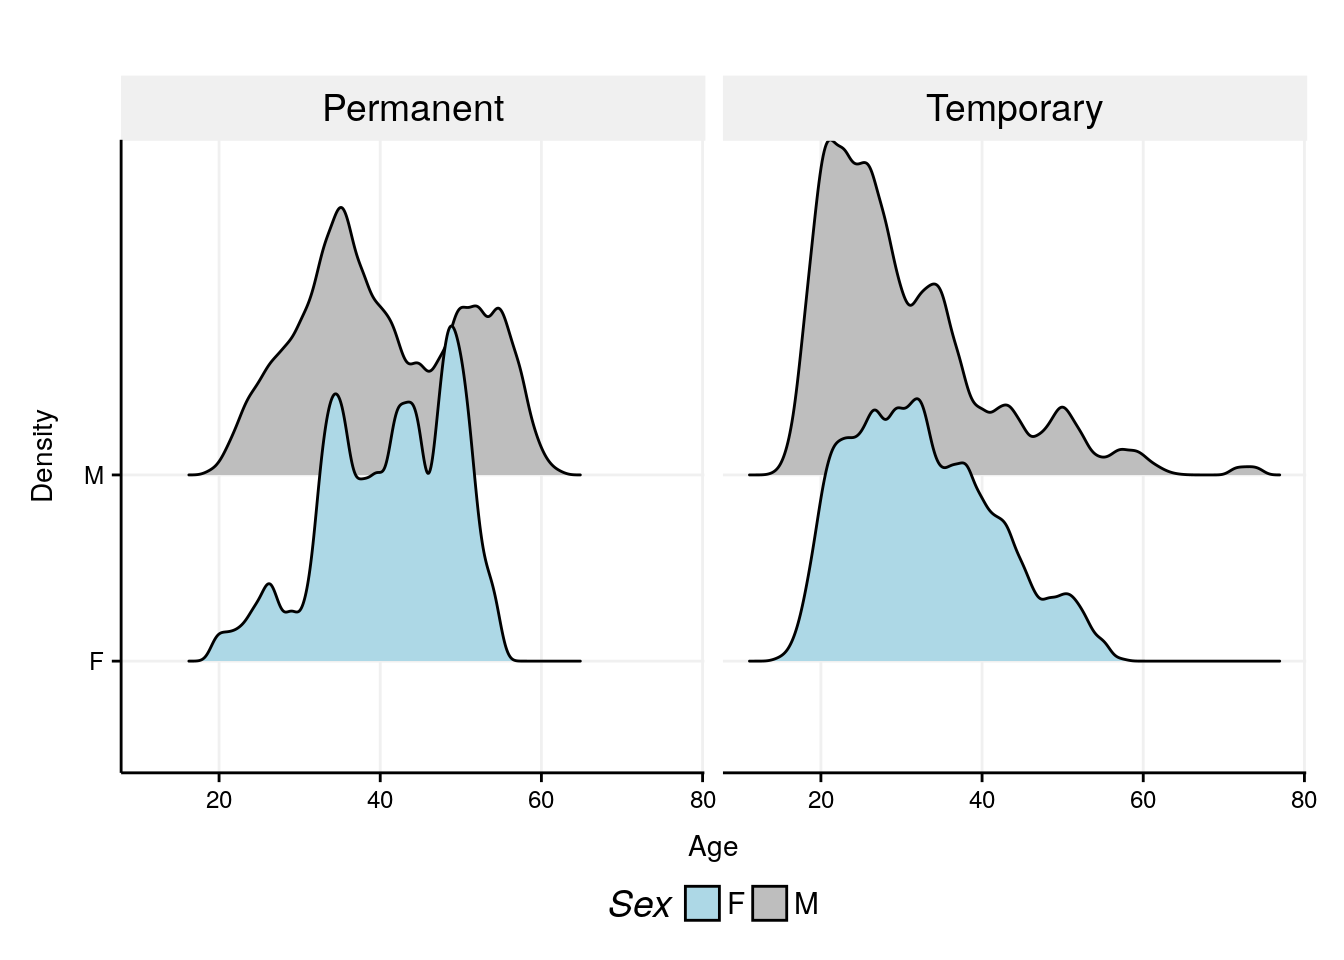
\includegraphics{figures/unnamed-chunk-13-1.pdf}
\caption{Clinical malaria (district of Manhiça), all-cause absenteeism
among Maragra workers, sick absenteeism among Maragra workers, estimated
rainfall, positive cases at company clinic, and test positivity rate at
company clinic}
\end{figure}

\textbf{Fumigations}: During the period from January 1st, 2012 through
December 31st, 2016, the Maragra Malaria Control Unit carried out 11,567
episodes of fumigation of residential ``agregados'' (household
combinations), for a total of 13,937 building-fumigation combinations.
The total number of unique agregados sprayed during this period was
4,045. Among the 3,362 workers for whom we have reliable absenteeism and
residential data, 692 had their homes fumigated at least once (the
majority of workers live off of the facility).

\textbf{Absences}: We observed 1,759,100 unique worker-days among the
3,362 workers. The all-period average absenteeism rate was 5.56\%,
though this rate varied widely as a function of worker department, sex,
residence, and season (table 1).

\begin{table}[ht]
\centering
\begin{tabular}{rlllll}
  \hline
Variable &  & 2013 & 2014 & 2015 & 2016 \\ 
  \hline
Malaria season & Low & 5.2\% & 7\% & 5.4\% & 3.3\% \\ 
   & High & 8.2\% & 12.8\% & 6.3\% & 2.7\% \\ 
  Worker type & Field worker & 4.4\% & 7.6\% & 3.9\% & 1.7\% \\ 
   & Not field worker & 10.7\% & 12.4\% & 11.5\% & 9.6\% \\ 
  Contract & Permanent & 12.1\% & 12.6\% & 12\% & 10.2\% \\ 
   & Temporary & 0.1\% & 5\% & 2.3\% & 0.5\% \\ 
  Sex & F & 4\% & 8.1\% & 4.4\% & 1.9\% \\ 
   & M & 8.1\% & 10\% & 6.5\% & 3.7\% \\ 
  Residence & Off site & 6.4\% & 9.6\% & 5.9\% & 3\% \\ 
   & On site & 9.4\% & 9.7\% & 6.1\% & 3.1\% \\ 
  Precipitation & Dry & 5.4\% & 7.7\% & 4.8\% & 2.4\% \\ 
   & Rainy & 7.9\% & 10.6\% & 7\% & 3.3\% \\ 
   \hline
\end{tabular}
\caption{Absenteeism rate by year and worker characteristics} 
\end{table}

\textbf{Costs}: The malaria control program at Maragra has an annual
operating budget of approximately XX, which includes the purchase of
insecticide, the wages of IRS sprayers and drivers, transportation,
record-keeping, and general administrative costs. Assuming linearity in
costs, the program spends approximately XX per agregado sprayed. With
each agregado containing an average of 2.2 workers, this translates to a
cost of XX per worker protected per season. Much of the benefit of IRS
goes to non-worker residents of sprayed agregados (who constitute a
majority), but this benefit is purposefully ignored for this analysis.

Given the likelihood that clinical data does not fully capture all
malaria cases, we do not quantify the costs of malaria infection to the
company. Rather, we first estimate the reduction in absenteeism
attributible to IRS, and then quantify the savings associated with
prevented absences. Additionally, we calculate the clinical savings of
IRS by first estimating the share of absences which are associated with
an episode of clinical malaria, and then applying the clinical cost per
case to the equivalent share of prevented absences. We intentionally
ignore the savings accrued by the public health system, as well as the
likely utility gains in secondary realms such as school absenteeism,
producitivity, etc.

\textbf{Effect of IRS on absenteeism}: IRS is associated with a
year-long, significant reduction in absenteeism during the malaria
season (figure 2). As one would expect if the mechanism by which IRS
reduces absence is through reduced malaria infection, the effect of IRS
during the low transmission season is significant, but far less
substantial in effect size.

\begin{figure}
\centering
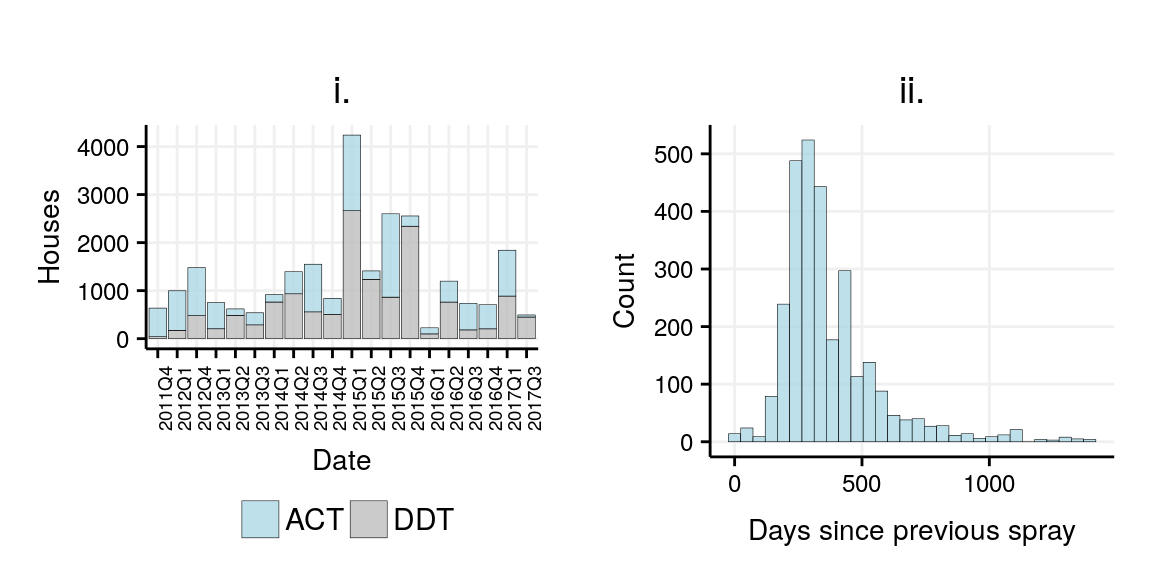
\includegraphics{figures/unnamed-chunk-16-1.pdf}
\caption{Estimated effect of IRS on absenteeism by season}
\end{figure}

We create 4 worker fixed effects models. Different models for field vs
not field, permanent vs temporary.

\begin{table}

\caption{\label{tab:unnamed-chunk-17}Models with worker fixed effects}
\centering
\begin{tabular}[t]{ll}
\toprule
Term & Estimate\\
\midrule
\addlinespace[1.5em]
\multicolumn{2}{l}{\textbf{Permanent field worker}}\\
\hspace{1em}Off site & 9.142 (P<0.001)\\
\hspace{1em}On site & 11.424 (P<0.001)\\
\hspace{1em}Malaria season & 3.424 (P<0.001)\\
\hspace{1em}Months since IRS: 01 & 3.831 (P<0.001)\\
\hspace{1em}Months since IRS: 02-04 & 4.199 (P<0.001)\\
\hspace{1em}Months since IRS: 05-09 & -3.194 (P<0.001)\\
\hspace{1em}Months since IRS: 10+ & -5.794 (P<0.001)\\
\hspace{1em}Malaria season:Months since IRS: 01 & -4.534 (P<0.001)\\
\hspace{1em}Malaria season:Months since IRS: 02-04 & -8.392 (P<0.001)\\
\hspace{1em}Malaria season:Months since IRS: 05-09 & -3.85 (P<0.001)\\
\hspace{1em}Malaria season:Months since IRS: 10+ & 4.504 (P=0.002)\\
\addlinespace[1.5em]
\multicolumn{2}{l}{\textbf{Permanent not field worker}}\\
\hspace{1em}Off site & 10.862 (P<0.001)\\
\hspace{1em}On site & 9.555 (P<0.001)\\
\hspace{1em}Malaria season & 2.077 (P<0.001)\\
\hspace{1em}Months since IRS: 01 & -2.083 (P<0.001)\\
\hspace{1em}Months since IRS: 02-04 & 3.904 (P<0.001)\\
\hspace{1em}Months since IRS: 05-09 & -0.834 (P=0.084)\\
\hspace{1em}Months since IRS: 10+ & -0.268 (P=0.742)\\
\hspace{1em}Malaria season:Months since IRS: 01 & 2.735 (P<0.001)\\
\hspace{1em}Malaria season:Months since IRS: 02-04 & -5.768 (P<0.001)\\
\hspace{1em}Malaria season:Months since IRS: 05-09 & -2.441 (P<0.001)\\
\hspace{1em}Malaria season:Months since IRS: 10+ & 4.497 (P<0.001)\\
\addlinespace[1.5em]
\multicolumn{2}{l}{\textbf{Temporary field worker}}\\
\hspace{1em}Off site & 0.985 (P<0.001)\\
\hspace{1em}On site & 1.078 (P<0.001)\\
\hspace{1em}Malaria season & -0.017 (P=0.461)\\
\hspace{1em}Months since IRS: 01 & -0.4 (P<0.001)\\
\hspace{1em}Months since IRS: 02-04 & -0.547 (P<0.001)\\
\hspace{1em}Months since IRS: 05-09 & -0.554 (P<0.001)\\
\hspace{1em}Months since IRS: 10+ & -0.992 (P<0.001)\\
\hspace{1em}Malaria season:Months since IRS: 01 & -0.092 (P=0.62)\\
\hspace{1em}Malaria season:Months since IRS: 02-04 & 0.172 (P=0.256)\\
\hspace{1em}Malaria season:Months since IRS: 05-09 & 0.062 (P=0.657)\\
\hspace{1em}Malaria season:Months since IRS: 10+ & 0.068 (P=0.771)\\
\addlinespace[1.5em]
\multicolumn{2}{l}{\textbf{Temporary not field worker}}\\
\hspace{1em}Off site & 4.136 (P<0.001)\\
\hspace{1em}On site & 3.834 (P<0.001)\\
\hspace{1em}Malaria season & -0.292 (P=0.16)\\
\hspace{1em}Months since IRS: 01 & -1.456 (P=0.389)\\
\hspace{1em}Months since IRS: 02-04 & 0.608 (P=0.574)\\
\hspace{1em}Months since IRS: 05-09 & -0.869 (P=0.405)\\
\hspace{1em}Months since IRS: 10+ & 10.583 (P<0.001)\\
\hspace{1em}Malaria season:Months since IRS: 01 & 6.045 (P=0.002)\\
\hspace{1em}Malaria season:Months since IRS: 02-04 & 0.604 (P=0.667)\\
\hspace{1em}Malaria season:Months since IRS: 05-09 & -1.482 (P=0.284)\\
\hspace{1em}Malaria season:Months since IRS: 10+ & -10.636 (P<0.001)\\
\bottomrule
\end{tabular}
\end{table}

\subsection{Return on investment}\label{return-on-investment}

Details here on ROI calculation outcomes
\todo{Not done yet. In conversation with Eduardo from MC about getting more accurate costs}

\subsection{Robustness and
generalizability}\label{robustness-and-generalizability}

Two principal concerns call into question the results of our analysis.
First, the application of IRS to a workers house may be endogenous. To
check for this bla bla bla
\todo{As per Menno's suggestion, will add details here pertaining to whether IRS predicts absenteeism before it is applied}.
The second concern is that our quantification of consists is distorted
by the fact that we treat IRS operations as essentially linear in
nature, when in reality economies of scale, in-kind purchases and other
factors likely make the true cost-per-spraying
convex.\todo{Will address this with some sensitivity analysis}

\section{Discussion}\label{discussion}

Overall stuff

\subsection{Limitations}\label{limitations}

\subsection{Implications}\label{implications}

\section*{References}\label{references}
\addcontentsline{toc}{section}{References}

\hypertarget{refs}{}
\hypertarget{ref-Azemar2009}{}
Azemar, C., Desbordes, R., 2009. Public governance, health and foreign
direct investment in sub-saharan africa. Journal of African Economies
18, 667--709. \url{https://doi.org/10.1093/jae/ejn028}

\hypertarget{ref-Bennett_2017}{}
Bennett, A., Avanceña, A.L.V., Wegbreit, J., Cotter, C., Roberts, K.,
Gosling, R., 2017. Engaging the private sector in malaria surveillance:
A review of strategies and recommendations for elimination settings.
Malaria Journal 16. \url{https://doi.org/10.1186/s12936-017-1901-1}

\hypertarget{ref-Bloom2008}{}
Bloom, D., Canning, D., 2008. Population Health and Economic Growth
1--25.

\hypertarget{ref-brewgit}{}
Brew, J., 2017. Malaria and sugar: An in-depth examination of the effect
of malaria control activities on the health and productivity of maragra
sugarcane factory workers. GitHub repository.

\hypertarget{ref-World1999}{}
Brundtland, G.H., 1999. WHO on Health and Economic Productivity 25,
396--402.

\hypertarget{ref-Buur2012}{}
Buur, L., Tembe, C.M., Baloi, O., 2012. The white gold: The role of
government and state in rehabilitating the sugar industry in mozambique.
Journal of Development Studies 48, 349--362.
\url{https://doi.org/10.1080/00220388.2011.635200}

\hypertarget{ref-CastelBranco2014}{}
Castel-Branco, C.N., 2014. Growth, capital accumulation and economic
porosity in mozambique: Social losses, private gains. Review of African
Political Economy 41, S26--S48.
\url{https://doi.org/10.1080/03056244.2014.976363}

\hypertarget{ref-German2013}{}
German, L., Schoneveld, G., Mwangi, E., 2013. Contemporary processes of
large-scale land acquisition in sub-saharan africa: Legal deficiency or
elite capture of the rule of law? World Development 48, 1--18.
\url{https://doi.org/10.1016/j.worlddev.2013.03.006}

\hypertarget{ref-Goodman1999}{}
Goodman, C., Coleman, P., Mills, A., 1999. Cost-effectiveness of malaria
control in sub-saharan africa. The Lancet 354, 378--385.
\url{https://doi.org/10.1016/s0140-6736(99)02141-8}

\hypertarget{ref-Han}{}
Han, L., 2015. Malaria in Mozambique: trialling payment by results.

\hypertarget{ref-Hanson2004}{}
Hanson, K., 2004. Public and private roles in malaria control: The
contributions of economic analysis. The American Journal of Tropical
Medicine and Hygiene 71, 168--173.

\hypertarget{ref-Howard_2017}{}
Howard, N., Guinness, L., Rowland, M., Durrani, N., Hansen, K.S., 2017.
Cost-effectiveness of adding indoor residual spraying to case management
in afghan refugee settlements in northwest pakistan during a prolonged
malaria epidemic. PLOS Neglected Tropical Diseases 11, e0005935.
\url{https://doi.org/10.1371/journal.pntd.0005935}

\hypertarget{ref-estatistica2009}{}
INE, 2011. Demographic health survey.

\hypertarget{ref-Kaula_2017}{}
Kaula, H., Buyungo, P., Opigo, J., 2017. Private sector role, readiness
and performance for malaria case management in uganda, 2015. Malaria
Journal 16. \url{https://doi.org/10.1186/s12936-017-1824-x}

\hypertarget{ref-Lee2017}{}
Lee, B.Y., Zenkov, E., Chatterjee, C., Candrinho, B., Zhang, S.,
Colborn, J., Briët, O.J.T., Brown, S.T., Mendis, C., Bartsch, S.M.,
Viisainen, K., DePasse, J.V., Stone, N.T.B., 2017. The economic value of
long-lasting insecticidal nets and indoor residual spraying
implementation in mozambique. The American Journal of Tropical Medicine
and Hygiene 96, 1430--1440. \url{https://doi.org/10.4269/ajtmh.16-0744}

\hypertarget{ref-Lopez_Bernal_2016}{}
Lopez Bernal, J., Cummins, S., Gasparrini, A., 2016. Interrupted time
series regression for the evaluation of public health interventions: A
tutorial. International Journal of Epidemiology dyw098.
\url{https://doi.org/10.1093/ije/dyw098}

\hypertarget{ref-McCarthy_2000}{}
McCarthy, D., Wolf, H., Wu, Y., 2000. The growth costs of malaria.
\url{https://doi.org/10.3386/w7541}

\hypertarget{ref-Moonasar_2016}{}
Moonasar, D., Maharaj, R., Kunene, S., Candrinho, B., Saute, F.,
Ntshalintshali, N., Morris, N., 2016. Towards malaria elimination in the
mosaswa (mozambique, south africa and swaziland) region. Malaria Journal
15. \url{https://doi.org/10.1186/s12936-016-1470-8}

\hypertarget{ref-Mouzin2011}{}
Mouzin, E., al., E., 2011. Business Investing in Malaria Control:
Economic Returns and a Healthy Workforce for Africa. Progress \& Impact
series.

\hypertarget{ref-Nhacolo_2006}{}
Nhacolo, A.Q., Nhalungo, D.A., Sacoor, C.N., Aponte, J.J., Thompson, R.,
Alonso, P., 2006. Levels and trends of demographic indices in southern
rural mozambique: Evidence from demographic surveillance in manhiça
district. BMC Public Health 6.
\url{https://doi.org/10.1186/1471-2458-6-291}

\hypertarget{ref-Nonvignon_2016}{}
Nonvignon, J., Aryeetey, G.C., Malm, K.L., Agyemang, S.A., Aubyn,
V.N.A., Peprah, N.Y., Bart-Plange, C.N., Aikins, M., 2016. Economic
burden of malaria on businesses in ghana: A case for private sector
investment in malaria control. Malaria Journal 15.
\url{https://doi.org/10.1186/s12936-016-1506-0}

\hypertarget{ref-Orem_2012}{}
Orem, J., Kirigia, J., Azairwe, R., Kasirye, I., Walker, O., 2012.
Impact of malaria morbidity on gross domestic product in uganda.
International Archives of Medicine 5, 12.
\url{https://doi.org/10.1186/1755-7682-5-12}

\hypertarget{ref-Purdy_2013}{}
Purdy, M., Rublin, D., Wei, K., Robinson, M., 2013. The economic case
for combating malaria. The American Journal of Tropical Medicine and
Hygiene 89, 819--823. \url{https://doi.org/10.4269/ajtmh.12-0689}

\hypertarget{ref-R}{}
R Core Team, 2017. R: A language and environment for statistical
computing. R Foundation for Statistical Computing, Vienna, Austria.

\hypertarget{ref-Robbins2012}{}
Robbins, G., Perkins, D., 2012. Mining fdi and infrastructure
development on africa's east coast: Examining the recent experience of
tanzania and mozambique. Journal of International Development 24,
220--236. \url{https://doi.org/10.1002/jid.2817}

\hypertarget{ref-Sachs2002}{}
Sachs, J., Malaney, P., 2002. The economic and social burden of malaria.
Nature 415, 680--685. \url{https://doi.org/10.1038/415680a}

\hypertarget{ref-Shretta2016}{}
Shretta, R., Avanceña, A.L.V., Hatefi, A., 2016. The economics of
malaria control and elimination: A systematic review. Malaria Journal
15. \url{https://doi.org/10.1186/s12936-016-1635-5}

\hypertarget{ref-Shretta_2017}{}
Shretta, R., Baral, R., Avanceña, A.L.V., Fox, K., Dannoruwa, A.P.,
Jayanetti, R., Jeyakumaran, A., Hasantha, R., Peris, L., Premaratne, R.,
2017. An investment case to prevent the reintroduction of malaria in sri
lanka. The American Journal of Tropical Medicine and Hygiene 16--0209.
\url{https://doi.org/10.4269/ajtmh.16-0209}

\hypertarget{ref-Vecchi_2013}{}
Vecchi, V., Hellowell, M., Gatti, S., 2013. Does the private sector
receive an excessive return from investments in health care
infrastructure projects? Evidence from the uk. Health Policy 110,
243--270. \url{https://doi.org/10.1016/j.healthpol.2012.12.010}

\hypertarget{ref-White_2011}{}
White, M.T., Conteh, L., Cibulskis, R., Ghani, A.C., 2011. Costs and
cost-effectiveness of malaria control interventions - a systematic
review. Malaria Journal 10, 337.
\url{https://doi.org/10.1186/1475-2875-10-337}

\hypertarget{ref-whoprof}{}
WHO, 2015. Malaria profile: Mozambique.

\hypertarget{ref-Winkler}{}
Winkler, D., 2013. Potential and Actual FDI Spillovers in Global Value
Chains.


\end{document}
